\documentclass[10pt,a4paper]{article}
\usepackage[latin1]{inputenc}
\usepackage{amsmath}
\usepackage{amsfonts}
\usepackage{amssymb}
\usepackage{lscape}
\usepackage{graphicx}
\author{Wendy Moniuk - 996659343}
\title{CSC343 Assignment 3}
\begin{document}
\begin{enumerate}

\item I am assuming that emails are unique among guests and hosts.

Every country and every city in my database has at least one guest and at least one host.

A host may have had no guests or many guests that have requested a couchsurf. A guest may have sent none or many couchsurf requests.

A member may have many friends or no friends.

A event may have zero invites or many invites associated with it. A member could be invited to zero or many events.

An event may have nobody going to it, or many going. A member could go to no events or many events.

A group must have at least one member.

A member can join zero or more groups.

A group may have zero or more messages. A member can post no messages or many messages. A post must be associated with at least one member and at least one group



\item See figure.
\begin{figure}
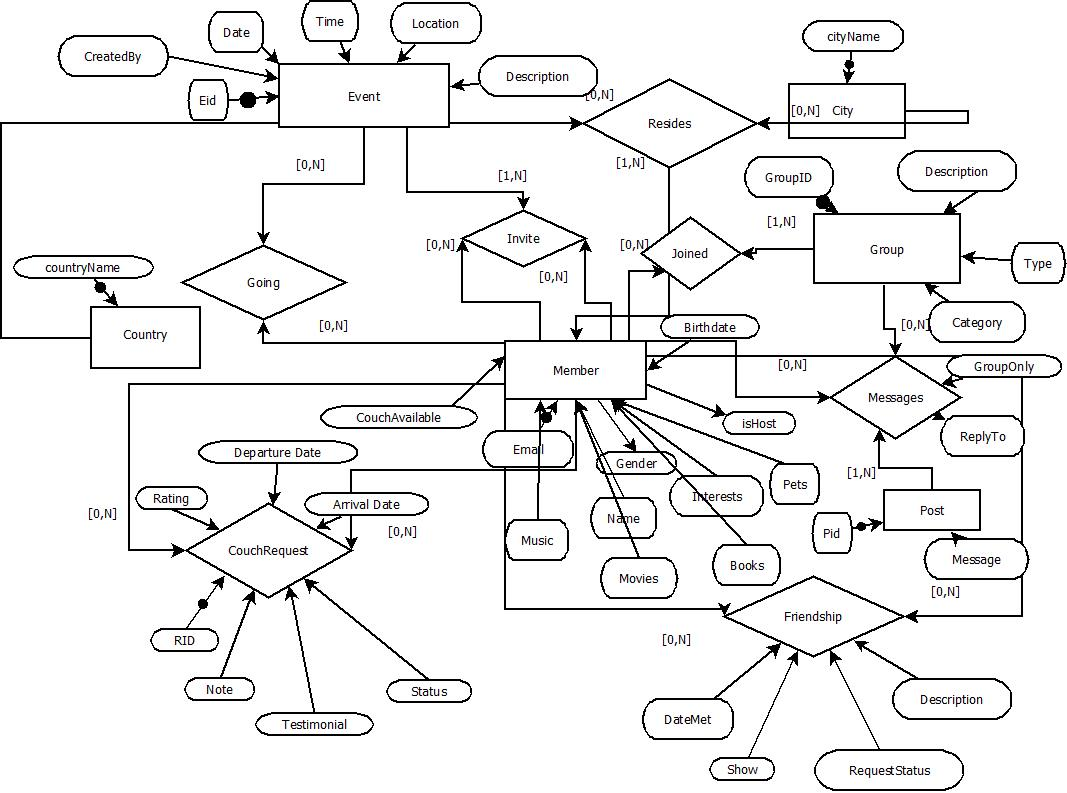
\includegraphics[width=5.5in]{./Diagram1}
\end{figure}

\item Member(\underline{email}, gender, birthdate, isHost, name, pets, interests, music, movies, couchAvailable)

Country(\underline{countryName})

City(\underline{cityName})

Group(\underline{GroupID}, Desc, type, category)

Event(\underline{Eid}, CreatedBy, date, time, location, description)

Post(\underline{pid}, message)

CouchRequest(\underline{RID}, guest, host, status, deptartureDate, arrivalDate, rating, note, testimonial)

Residesin(\underline{mid}, \underline{country}, \underline{city})

Friendship(\underline{member1}, \underline{member2}, dateMet, Show, RequestStatus, Description)

Joined(\underline{mid}, \underline{groupID})

Messages(\underline{mid}, \underline{pid}, \underline{groupID}, groupOnly, replyTo)

Invite(\underline{eid}, \underline{inviter}, \underline{invitee})

Going(\underline{eid}, \underline{mid})

CouchRequest(guest) $\subseteq$ $\pi_{email}\sigma_{isHost = false}$Member

CouchRequest(host) $\subseteq$ 
$\pi_{email}\sigma_{isHost = true}$Member

Event(CreatedBy) $\subseteq$ Member(email)

Residesin(mid) $\subseteq$ Member(email)

Residesin(country) $\subseteq$ Country(countryName)

Residesin(city) $\subseteq$ City(cityName)

Friendship(member1) $\subseteq$ Member(email)

Friendship(member2) $\subseteq$ Member(email)

Joined(mid) $\subseteq$ Member(email)

Joined(groupID) $\subseteq$ Group(GroupID)

Messages(mid) $\subseteq$ Member(email)

Messages(pid) $\subseteq$ Post(pid)

Messages(groupID) $\subseteq$ Group(GroupID)

Invite(eid) $\subseteq$ Event(eid)

Invite(inviter) $\subseteq$ Member(email)

Invite(invitee) $\subseteq$ Member(email)

Going(eid) $\subseteq$ Event(eid)

Going(mid) $\subseteq$ Member(email)

$\sigma_{rating>5 \bigvee rating < 1}$CouchRequest $\subseteq \emptyset$

\item

\begin{verbatim}
CREATE TABLE member{
email varchar(50) PRIMARY KEY,
gender char,
birthdate date,
isHost boolean,
name varchar(50),
pets varchar(30),
interests varchar(50),
music varchar(50),
movies varchar(50), 
couchAvailable boolean
};

CREATE TABLE country{
countryName varchar(20) PRIMARY KEY
};

CREATE TABLE city{
cityName varchar(20) PRIMARY KEY
};

CREATE TABLE group(
groupid integer PRIMARY KEY,
desc varchar(100),
type char(7), CHECK type = 'PRIVATE' OR type = 'PUBLIC',
category varchar(20)
);

CREATE TABLE event(
eid integer PRIMARY KEY,
createdBy varchar(50) REFERENCES member(email),
date date NOT NULL,
time time NOT NULL,
location varchar(50) NOT NULL,
description varchar(100)
);

CREATE TABLE post(
pid integer PRIMARY KEY,
message varchar(300)
);

CREATE TABLE couchrequest(
rid integer PRIMARY KEY,
guest varchar(50) REFERENCES member(email),
host varchar(50) REFERENCES memver(email),
status char(8),
CHECK status = 'ACCEPTED' or status = 'PENDING' or status = 'DECLINED'
 or status = 'MAYBE',
departureDate date,
arrivalDate date, 
rating integer,
CHECK rating >=1 and rating <=5,
note varchar(50),
testimonial varchar(100)
);

CREATE TABLE residesin(
mid varchar(50) REFERENCES member(email),
country varchar(20) REFERENCES country,
city varchar(20) REFERENCES city
);

CREATE TABLE friendship(
member1 varchar(50) REFERENCES member(email),
member2 varchar(50) REFERENCES member(email),
dateMet date,
show boolean,
requeststatus char(5),
check requeststatus = 'YES' or requeststatus = 'NO' 
or requeststatus = 'MAYBE',
description varchar(100)
);

CREATE TABLE joined(
mid varchar(50) REFERENCES member(email),
groupID integer REFERENCES group
);

CREATE TABLE messages(
mid varchar(50) REFERENCES member(email),
pid integer REFERENCES post,
groupID integer REFERENCES group,
grouponly boolean,
replyto integer,
);

CREATE TABLE invite(
eid integer REFERENCES event,
inviter varchar(50) REFERENCES member(email),
invitee varchar(50) REFERENCES member(email)
);

CREATE TABLE going(
eid integer REFERENCES event,
mid varchar(50) REFERENCES member(email)
);
\end{verbatim}
\end{enumerate}
\end{document}